\section{氧气的性质和用途}\label{sec:1-2}

我们已经知道,氧气约占空气体积的 $1/5$,它跟人类关系很密切,是人的生命不可缺少的物质。
过去,人们曾把氧气叫做 “养气”。

我们要研究氧气,首先要认识氧气的性质。

\subsection{氧气的性质}

\begin{wrapfigure}[11]{r}{5cm}
    \centering
    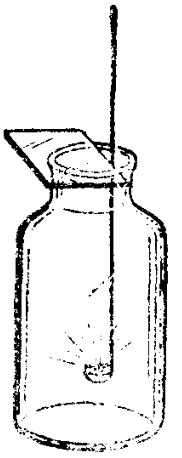
\includegraphics[width=2cm]{../pic/czhx1-ch1-3}
    \caption{木炭在氧气里燃烧}\label{fig:1-3}
\end{wrapfigure}

1. 物理性质

在通常状况下,氧气是一种没有颜色、没有气味的气体。它不易溶解于水,$1$ 升水只能溶解大约 $30$ 毫升的氧气。
在标准状况\footnote{标准状况指的是在 $0$ ℃ 左右和 $1$ 标准大气压时的状况。}下,
氧气的密度是 $1.429$ 克/升,比空气略大(空气的密度 $1.293$ 克/升)。

在 $1$ 标准大气压下,氧气在 $-183$ ℃ 时变为淡蓝色的液体,在 $-218$ ℃ 时变成雪花状的淡蓝色的固体。

2. 化学性质

让我们先来做几个实验。

\begin{shiyan}
    把一小块木炭放在燃烧匙里,伸进盛有氧气的集气瓶里,观察木炭是否燃烧。
    再把木炭加热到发红,然后连炭带燃烧匙伸进盛有氧气的集气瓶里,观察木炭燃烧时发生的现象。
    注意木炭在空气里和在氧气里燃烧有什么不同(图\ref{fig:1-3})。
    等燃烧停止后,立即向瓶内倒进一些澄清的石灰水,振荡,观察石灰水发生什么变化。
\end{shiyan}



木炭(主要成分是碳)在氧气里燃烧比在空气里更旺,发出白光、并放出热量。
燃烧后生成的无色气体能使澄清的石灰水变浑浊,证明这种气体是二氧化碳。
这个实验说明碳跟氧气起反应,生成了二氧化碳。这个化学反应可以表示如下:
\begin{fangchengshi}
    \ce{\text{碳} + \text{氧气} ->[\text{点燃}] \text{二氧化碳}}
\end{fangchengshi}


\begin{wrapfigure}[16]{r}{5cm}
    \centering
    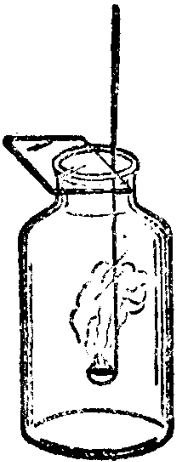
\includegraphics[width=2cm]{../pic/czhx1-ch1-4}
    \caption{硫在氧气里燃烧}\label{fig:1-4}
\end{wrapfigure}

\wrapfiguretrick

\begin{shiyan}
    在燃烧匙里放少量硫,加热,直到发生燃烧,观察硫在空气里燃烧时发生的现象。
    然后把带燃着的硫的燃烧匙伸进盛有氧气的集气瓶里,再观察硫在氧气里燃烧时发生的现象(图 \ref{fig:1-4})。
    比较硫在空气和在氧气里燃烧有什么不同。
\end{shiyan}

硫在空气里燃烧发出微弱的淡蓝色火焰,而在氧气里燃烧更旺,发出明亮的蓝紫色火焰。
硫跟氧气发生了化学反应,生成一种叫二氧化硫的有刺激性气味的气体,并放出热量。
这个化学反应可以表示如下:

\vspace*{-1em}\begin{fangchengshi}
    \ce{\text{硫} + \text{氧气} ->[\text{点燃}] \text{二氧化硫}}
\end{fangchengshi}

氧气还能跟磷起反应,生成一种叫五氧化二磷的白色固体。
\begin{fangchengshi}
    \ce{\text{磷} + \text{氧气} ->[\text{点燃}] \text{五氧化二磷}}
\end{fangchengshi}

氧气除了能够跟碳、硫、磷等这些易燃烧的物质起反应外,是否能够跟铁等物质起反应,发生燃烧现象?

我们知道,铁在空气里是不会燃烧的,那么,铁在氧气里能不能发生燃烧现象呢?

\begin{wrapfigure}[14]{r}{5cm}
    \centering
    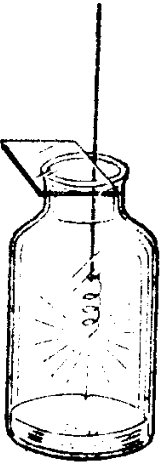
\includegraphics[width=2cm]{../pic/czhx1-ch1-5}
    \caption{铁在氧气里燃烧}\label{fig:1-5}
\end{wrapfigure}

\wrapfiguretrick


\begin{shiyan}
    把光亮的细铁线绕成螺旋状,一端系在一根铁丝上,另一端系上一根火柴,点燃火柴后,
    立即连火柴带细铁丝伸进盛有氧气的集气瓶里,观察发生的现象(图 \ref{fig:1-5} )。
    集气瓶里要预先装少量水或在瓶底铺上一层细沙,为什么?

\end{shiyan}

细铁丝在氧气里剧烈燃烧,火星四射,生成了一种叫四氧化三铁的黑色固体。
生成物熔化后溅落下来,证明燃烧时放出大量的热。
为了防止溅落的熔化物炸裂瓶底,所以瓶里要预先装少量水或在瓶底铺上一薄层细沙。

这个化学反应可以表示如下:
\begin{fangchengshi}
    \ce{\text{铁} + \text{氧气} ->[\text{点燃}] \text{四氧化三铁}}
\end{fangchengshi}

不仅铁能跟氧气发生化学反应,而且铝、铜等也能跟氧气发生化学反应。

上面这些反应,都是由两种物质生成另一种物质的化学反应,我们把
\zhongdian{由两种或两种以上的物质生成另一种物质的反应,叫做化合反应。}


除碳、硫、铁等物质外,还有哪些物质也可以在氧气里燃烧呢?

\begin{wrapfigure}[11]{r}{5cm}
    \centering
    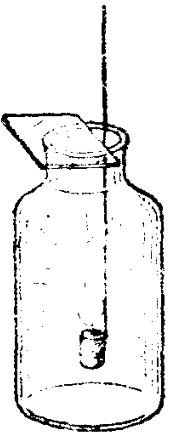
\includegraphics[width=2cm]{../pic/czhx1-ch1-6}
    \caption{蜡烛在氧气里燃烧}\label{fig:1-6}
\end{wrapfigure}

\wrapfiguretrick


\begin{shiyan}
    把点燃的蜡烛伸进盛有氧气的集气瓶里,观察并比较蜡烛在空气里和在氧气里燃烧有什么不同(图 \ref{fig:1-6})。
    燃烧停止后,等稍冷却,观察瓶壁上有什么出现。
    取出蜡烛,向瓶里倒进一些澄清的石灰水,振荡,石灰水有什么变化。

\end{shiyan}

蜡烛在氧气里燃烧比在空气里更旺,发出白光,并放出热量。
瓶壁上有水雾出现。倒进瓶里的澄清石灰水变浑浊。
这个实验说明蜡烛(主要成分是含有碳和氢的石蜡)跟氧气起反应,生成了水和二氧化碳。
这个反应是化合反应吗?

其它象煤、木材、酒精、汽油等物质在空气里燃烧,也就是这些物质跟空气里的氧气发生化学反应。

碳、硫、铁、蜡烛等在氧气里燃烧,发生了化学反应。这些反应里,有的是化合反应,有的不是化合反应。
但它们有一个共同的特点,就是物质跟氧气发生反应。我们把物质跟氧发生的化学反应叫做\zhongdian{氧化反应}。

我们从以上的事实可以认识到,氧气是一种化学性质比较活泼的气体,它能够跟许多物质发生化学反应,
同时放出热量。这是氧气的重要性质。


\subsection{燃烧和缓慢氧化}

在生产和日常生活里,我们经常看到一些可燃物在空气里燃烧,这是一种剧烈的氧化反应。
我们通常讲的\zhongdian{燃烧}指的是可燃物跟空气的氧气发生的一种发热发光的剧烈的氧化反应。

由于空气里的氧气被不能支持燃烧的氮气冲淡,所以可燃物在空气里燃烧,远没有在纯净的氧气里燃烧那么剧烈。
因此,要使可燃物燃烧,必须要有充足的氧气。但是只有充足的氧气就能燃烧了吗?
从上面的实验知道,没有经过加热的木炭放在纯净的氧气里,木炭没有燃烧,而必须把红热的木炭放在氧气里,才能燃烧。
可见,物质燃烧除了需要氧气外,还要达到一定的温度才行。
在一般情况下,使物质着火燃烧所需要的最低温度叫做\zhongdian{着火点}。各种物质的着火点是各不相同的。


由此可知,要使可燃物燃烧,必须具备下列两个条件:

1. 跟氧气接触;

2. 温度达到着火点。

\taolun 根据可燃物燃烧的条件,你怎样使火熄灭?

某些可燃物在有限的空间里发生急速燃烧的时候,常会发生\textbf{爆炸}。

\begin{yuedu}

    粉状的或气态的可燃物如果跟空气充分混和,由于接触空气的总面积很大,温度达到了着火点,就会发生急速燃烧。
    要是这种燃烧发生在有限的空间里,在很短时间内聚集了产生的大量的热,就会使气态生成物的体积突然膨胀,引起爆炸。
    在面粉工厂和存放汽油等的仓库的墙上,常写有 “严禁烟火” 字样,
    就是因为这些地方的空气里常常混有可燃物质的小颗粒或蒸气,接触到火星有发生爆炸的危险。

\end{yuedu}

铁在氧气里燃烧是一种剧烈的氧化反应。
铁生锈也是一种氧化反应,但这种氧化反应进行得很缓慢,也不象燃烧那样剧烈地发热发光,甚至不易察觉。
我们把这种氧化叫做\zhongdian{缓慢氧化}。呼吸作用、食物的腐败等都包含缓慢氧化。

物质在缓慢氧化过程里也产生热。
如果在某种情况下热量不易散失,以致越积越多,温度逐渐升高,达到那种物质的着火点,
不经点火就会引起燃烧。这种由于缓慢氧化而引起的自发燃烧,叫做\zhongdian{自燃}。


\begin{wrapfigure}[11]{r}{5cm}
    \centering
    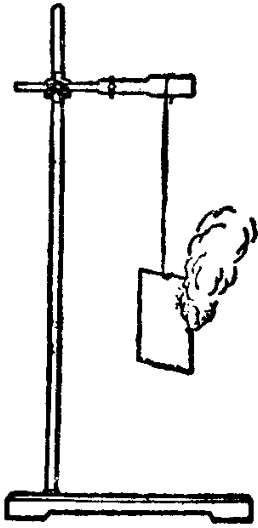
\includegraphics[width=2cm]{../pic/czhx1-ch1-7}
    \caption{白磷的自燃}\label{fig:1-7}
\end{wrapfigure}

\wrapfiguretrick

\begin{shiyan}
    把少量白磷溶解在二硫化碳里, 把这种液体滴一些在一小块滤纸上,然后把滤纸挂起晾干(图 \ref{fig:1-7}),
    观察发生的现象。不久,可以看到滤纸发火燃烧。滤纸为什么会自行燃烧起来呢?
\end{shiyan}

滤纸的燃烧是由白磷的自燃而引起的。
因为二硫化碳很容易挥发,滤纸上的二硫化碳挥发后,白磷就成为小粒附着在滤纸上,增大了跟空气接触的面积。
在这种情况下,小粒白磷就容易起缓慢氧化,产生的热量越积越多,
使温度上升到白磷的着火点(白磷的着火点很低,只有 $40$ ℃ ),发生自燃,烧着了滤纸。

\begin{yuedu}

    稻草、麦秆、煤炭、擦机器的破布等,如果堆放得不好,空气不流通,缓慢氧化产生的热不能及时散出,日久也会自燃。
    过去,有些人由于不懂自燃的科学道理,迷信地叫它为 “天火”。
    为了防止自燃现象发生,可燃的物质一般不要堆放得太多,并要注意通风或经常翻动。

    缓慢氧化产生的热可以利用在农业生产上。例如,把适量未经腐熟的马粪和猪、牛厩肥适当混和,
    埋在温室的土层下,能使土壤的温度升高,从而促进蔬菜的生长和发育。

    所以,对缓慢氧化的研究很有实际意义。

\end{yuedu}


\subsection{氧气的用途}

根据氧气很容易跟别的物质发生反应,同时放出热量的这种性质,人们已经把它广泛地应用在工农业生产、科学技术等方面。

一般情况下,燃烧和呼吸,只需要空气就行了。但在特殊情况下,需要纯净的氧气。

在钢铁工业上,把氧气或者添加了氧气的空气鼓入炼钢炉或炼铁炉,可以提高炉子里的温度,加速冶炼过程,提高钢铁的质量和产量。

利用氧炔吹管(图\ref{fig:1-8}),使乙炔\footnote{炔\,音\pinyin{que1}。乙炔是一种可燃性气体,俗名电石气。}
在氧气里燃烧,能产生一种叫做氧炔焰的火焰,温度可达 $3000$ ℃ 以上。

\begin{figure}[htbp]
    \centering
    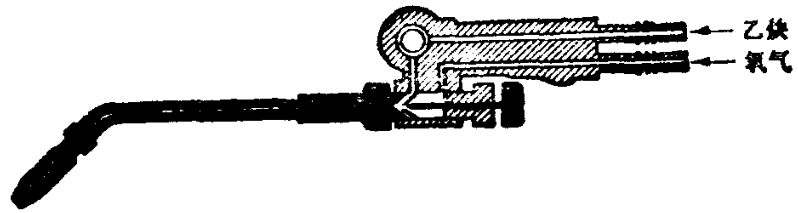
\includegraphics[width=9cm]{../pic/czhx1-ch1-8}
    \caption{氧炔吹管}\label{fig:1-8}
\end{figure}


这个化学反应可以表示如下:
\begin{fangchengshi}
    \ce{\text{乙炔} + \text{氧气} ->[\text{点燃}] \text{二氧化碳} + \text{水}}
\end{fangchengshi}

氧炔焰可以用来焊接或割断金属。

用液态氧浸渍多孔的可燃性物质,如木屑、木炭粉等,可以制成液氧炸药,用来开山采矿,开沟挖渠。

此外,液态氧还用在字宙火箭的发动机里,促使燃料迅速燃烧,推动火箭前进。

急救病人常常需要供给氧气,高空飞行员、潜水员、登山运动员以及其它在缺氧的场所工作的人员,都要携带供氧的设备。

\begin{xiti}

\xiaoti{下列关于氧气的物理性质的叙述,哪些是错误的?}
\begin{xiaoxiaotis}

    \xxt{氧气是没有颜色、没有气味的气体。}

    \xxt{液态氧是没有颜色的。}

    \xxt{氧气不易溶解于水。}

    \xxt{氧气的密度小于空气的密度。}

\end{xiaoxiaotis}


\xiaoti{怎样用简单的方法证明集气瓶里盛的是氧气而不是空气。}

\xiaoti{填空:}
\begin{xiaoxiaotis}

    \xxt{\ce{\text{碳} + \text{氧气} ->[\text{点燃}] \text{\ewkh[4em]}}}

    \xxt{\ce{\text{硫} + \text{氧气} ->[\text{点燃}] \text{\ewkh[4em]}}}

    \xxt{\ce{\text{铁} + \text{氧气} ->[\text{点燃}] \text{\ewkh[4em]}}}

    \xxt{\ce{\text{石蜡} + \text{氧气} ->[\text{点燃}] \text{\ewkh[4em]} + \text{\ewkh[4em]}}}

\end{xiaoxiaotis}

\xiaoti{下面列出六个化学反应:}
\begin{xiaoxiaotis}

    \xxt{\ce{\text{镁} + \text{氧气} ->[\text{点燃}] \text{氧化镁} }}

    \xxt{\ce{\text{碳酸氢铵} ->[\text{加热}] \text{氨气} + \text{水} + \text{二氧化碳} }}

    \xxt{\ce{\text{氢气} + \text{氧气} ->[\text{点燃}] \text{水} }}

    \xxt{\ce{\text{氨气} + \text{氯化氢} -> \text{氯化铵} }}

    \xxt{\ce{\text{乙炔} + \text{氧气} ->[\text{点燃}] \text{二氧化碳} + \text{水} }}

    \xxt{\ce{\text{氧化汞} ->[\text{加热}] \text{氧气} + \text{汞} }}

\end{xiaoxiaotis}

在这些化学反应里,属于化合反应的有 \xhx[5em],属于氧化反应的有 \xhx[5em]。

\xiaoti{在家里仔细观察一支点燃的蜡烛,并把观察的结果记录下来。}

\end{xiti}

